\begin{frame}{Mecánica del polarimetro}
    \begin{columns}
        \begin{column}{0.5\textwidth}
            \begin{figure}[H]
                \centering
                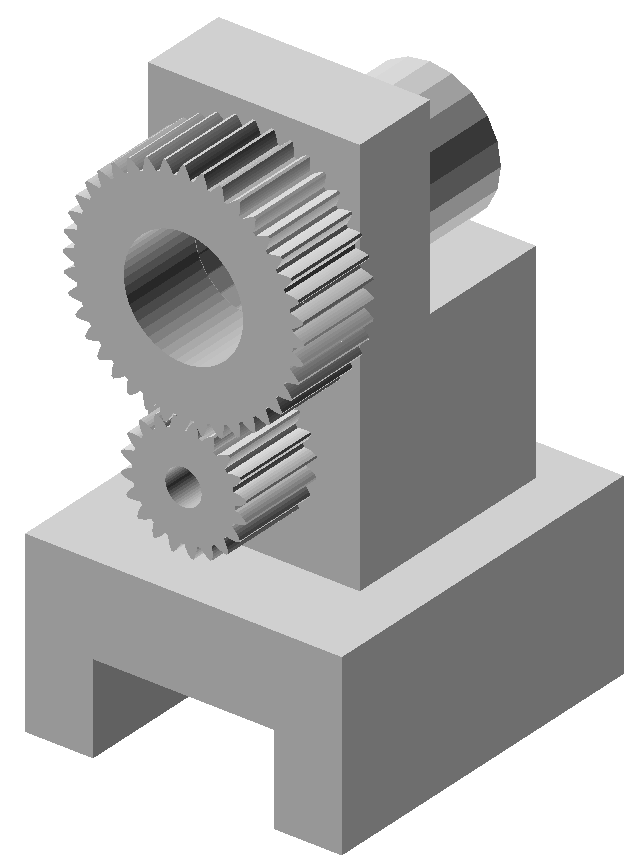
\includegraphics[width=0.8\textwidth]{fig/polarimetro/soporte_all}
                \label{fig:polarimetro/soporte_all}
            \end{figure}
        \end{column}
        \begin{column}{0.5\textwidth}
            \begin{itemize}
                \item Motor NEMA 8 mueve el engranaje inferior paso a paso
                \item Utiliza electrónica creada para el perfilador. Mide en cada paso del motor
                \item En el engranaje grande se monta una lámina polarizadora
            \end{itemize} 
        \end{column}
    \end{columns}
\end{frame}

\begin{frame}{Calibración de láminas polarizadoras}
        
        \begin{columns}
            \begin{column}{0.5\textwidth}
                \begin{figure}[H]
                \centering
                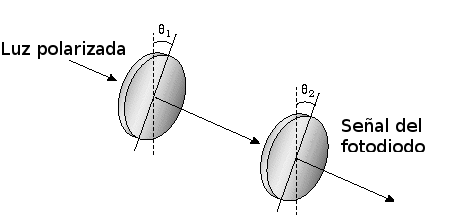
\includegraphics[width=\textwidth]{fig/polarimetro/calibracion}
                \label{fig:polarimetro_calibracion}
            \end{figure}
            \end{column}
            \begin{column}{0.5\textwidth}
                \begin{itemize}
                    \item Con dos polarizadores móviles se puede terminar los parámetros del material polarizador
                    \item El plástico usado tiene la siguiente matriz de transmisión $\begin{pmatrix} 0,5 & 0 \\ 0 & 2\times 10^{-6} \end{pmatrix}$
                \end{itemize}
            \end{column}
        \end{columns}
\end{frame}


\begin{frame}{Mediciones con el polarimetro}
    Medición de polarización par láser azul DHOM-M-473  
    \begin{columns}
        \begin{column}{0.5\textwidth}
            Antes de la fibra óptica
            \begin{figure}[H]
                \centering
                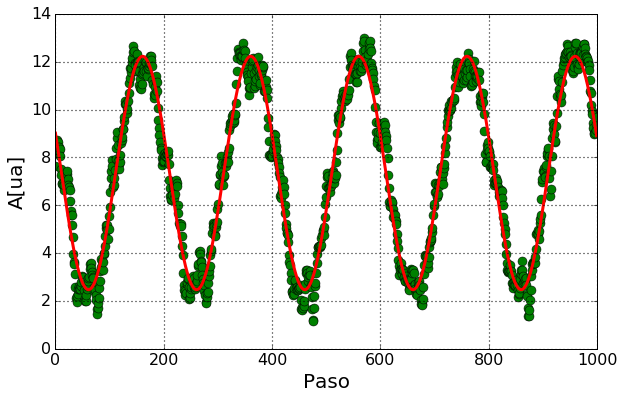
\includegraphics[width=\textwidth]{fig/polarimetro/polarizacion_azul}
                \label{fig:polarimetro_calibracion}
            \end{figure}
            $\frac{\max - \min}{\max + \min} = (0,664
 \pm 0,025)$
        \end{column}
        \begin{column}{0.5\textwidth}
        
            Después de la fibra óptica
            \begin{figure}[H]
                \centering
                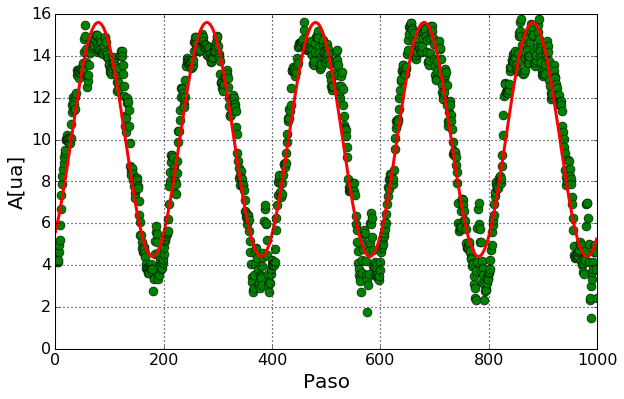
\includegraphics[width=\textwidth]{fig/polarimetro/polarizacion_azul_fibra}
                \label{fig:polarimetro_calibracion}
            \end{figure}
            $\frac{\max - \min}{\max + \min} = (0,660
 \pm 0,029)$
        \end{column}
    \end{columns}

\end{frame}
